\section{Data structure summary of the train and test data-sets}\label{appendix:datastruct}

\begin{table}[H]
\begin{tabular}{ |p{3cm}||p{3cm}|p{3cm}|p{3cm}|  }
 \hline
 \multicolumn{4}{|c|}{\textbf{Data structure}} \\
 \hline
 \rowcolor{lightgray} \footnotesize{\textbf{Data-set}}& \footnotesize{\textbf{\#Data-points}} & \footnotesize{\textbf{\#Unique species}} & \footnotesize{\textbf{Mean \#locs per species}}\\
 \hline
 \footnotesize{\textbf{Train}}   & \footnotesize{272037}    & \footnotesize{500} &   \footnotesize{544}\\
 \footnotesize{\textbf{Test}} &   \footnotesize{288122}  & \footnotesize{500}   &\footnotesize{3413}\\

 \hline
\end{tabular}
\caption{Data structure of the provided data-sets `train' and `test'.}
\label{tab:my_label}
\end{table}



\section{Species observation count per. continent}\label{appendix:table1}

\begin{table}[H]
\begin{tabular}{ |p{3cm}||p{3cm}|p{3cm}|p{3cm}|  }
 \hline
 \rowcolor{lightgray} \footnotesize{\textbf{Continents}}& \footnotesize{\textbf{\#Observations}} & \footnotesize{\textbf{\#Species}} & \footnotesize{\textbf{Average \#Observations per Species}}\\
 \hline
 \footnotesize{\textbf{N. America}}   & \footnotesize{126579}    & \footnotesize{134} &   \footnotesize{944.6}\\
 \footnotesize{\textbf{Europe}}   & \footnotesize{34774}    & \footnotesize{34} &   \footnotesize{1022.8}\\
 \footnotesize{\textbf{Oceania}}   & \footnotesize{35763}    & \footnotesize{73} &   \footnotesize{489.9}\\
 \footnotesize{\textbf{Asia}}   & \footnotesize{22317}    & \footnotesize{67} &   \footnotesize{333.1}\\
 \footnotesize{\textbf{Africa}}   & \footnotesize{32737}    & \footnotesize{122} &   \footnotesize{268.3}\\
 \footnotesize{\textbf{S. America}}   & \footnotesize{19659}    & \footnotesize{69} &   \footnotesize{284.9}\\
 \footnotesize{\textbf{Antarctica}}   & \footnotesize{208}    & \footnotesize{1} &   \footnotesize{208}\\
 \hline
\end{tabular}
\caption{Number of Observations, Number of Species ann Average Number of Observations per Species for each Continent.}

\end{table}


\section{Feed-Forward Neural Network Architecture} \label{appendix:ffnn}
\begin{figure}[h]
\centering
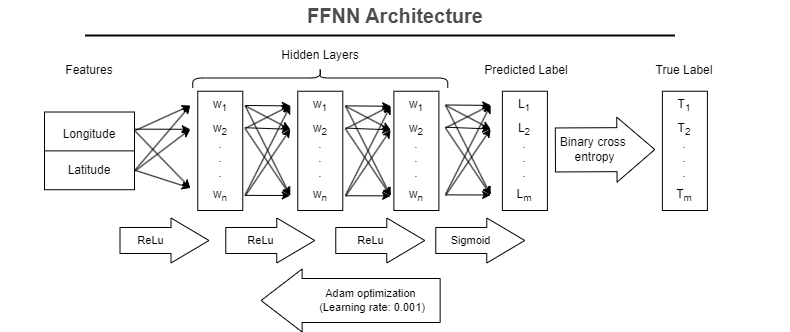
\includegraphics[width = .6\textwidth]{Images/neural_net.png}
\caption{Feed-forward neural network architecture used to predict species on location data.}
\label{FFNNarchitecture}
\end{figure}


\section{Random Forest Optimisation}\label{appendix:RFF1}

\begin{figure}[H]
\centering
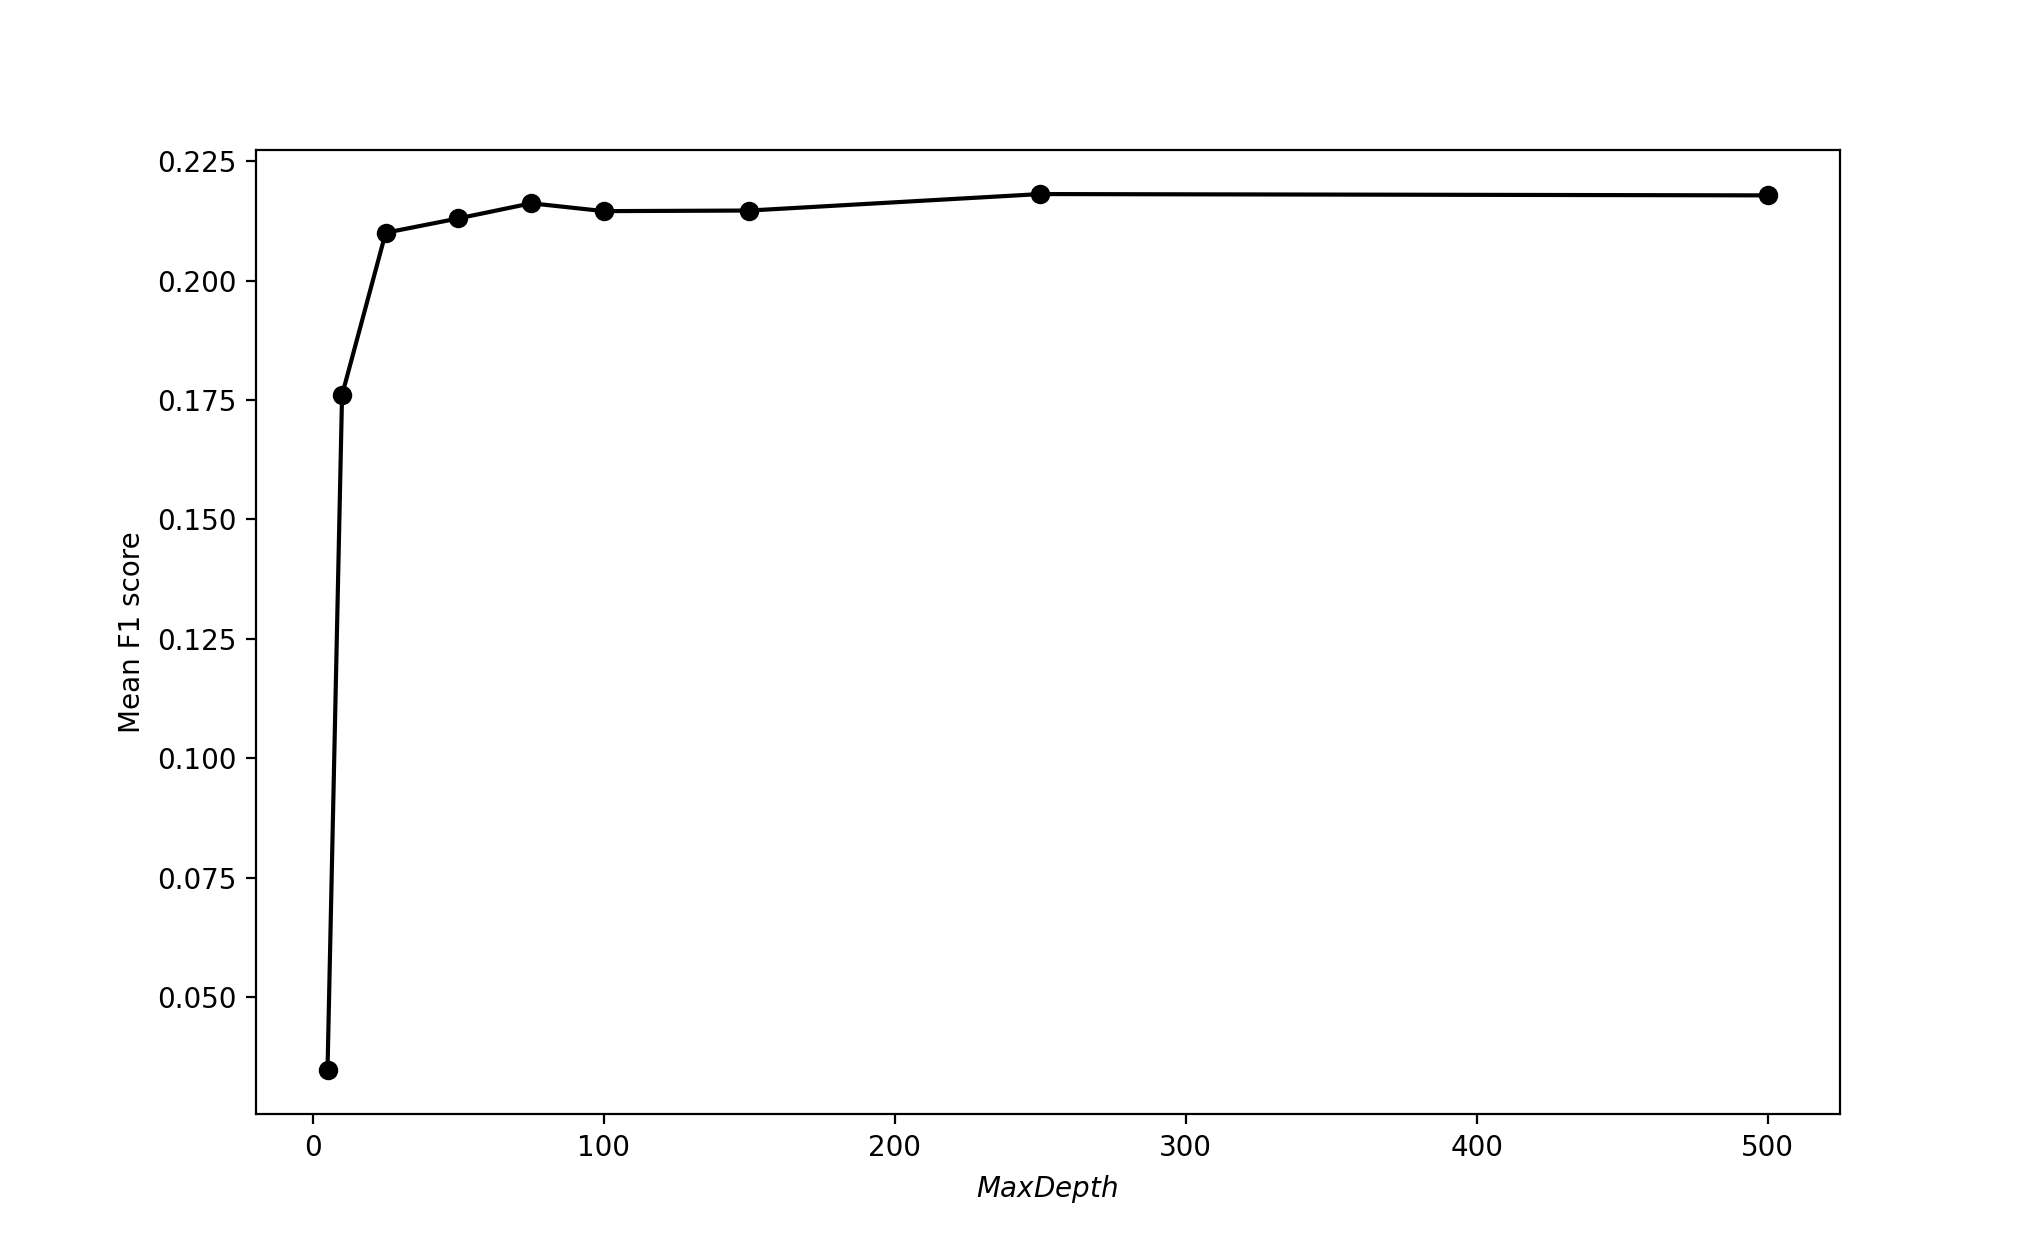
\includegraphics[width = .6\textwidth]{Images/Appendix.png}
\caption{Mean F1 score across all species for different values of maximum depth. At \textit{max\_depth=10} the F-score plateaus.}
\label{RFF1}
\end{figure}


\section{KNN Optimisation} \label{appendix:KNNF1}

\begin{figure}[H]
\centering
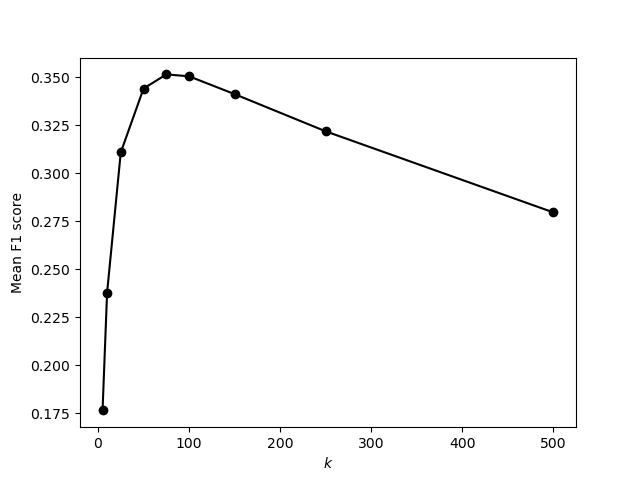
\includegraphics[width = .6\textwidth]{Images/knn_f1_scores.png}
\caption{Mean F1 score across all species for different values of k, the number of nearest neighbours used in KNN classification. The maximum value corresponds to $k = 75$.}
\label{KNNF1}
\end{figure}




\section{Bioclimatic variables} \label{appendix:bio}

\begin{figure}[H]
\label{appendix:extra}
\centering

\begin{subfigure}{.3\linewidth}
  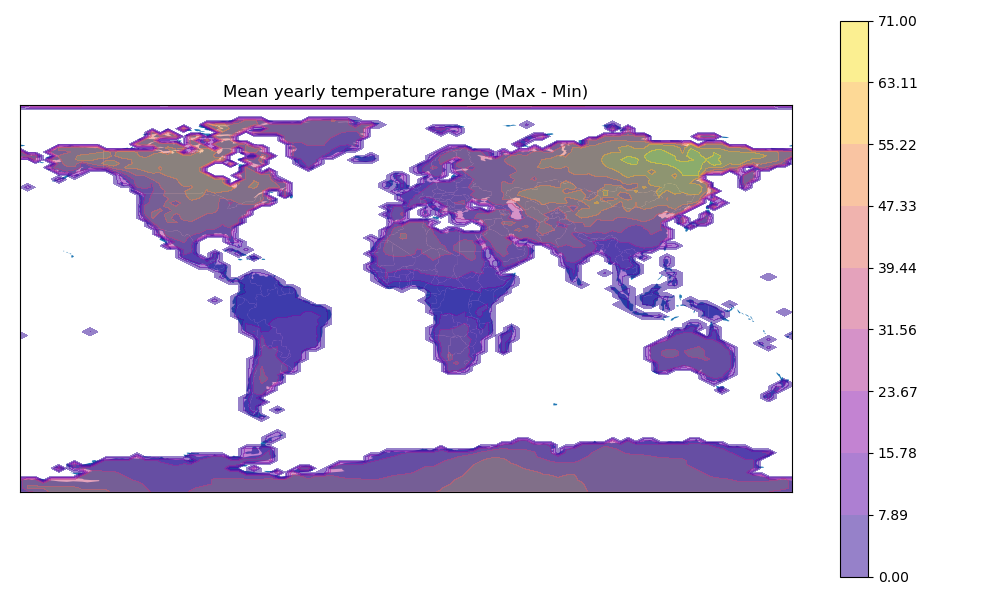
\includegraphics[width=\linewidth]{Images/mean_temp.png}

\end{subfigure}
\begin{subfigure}{.3\linewidth}
  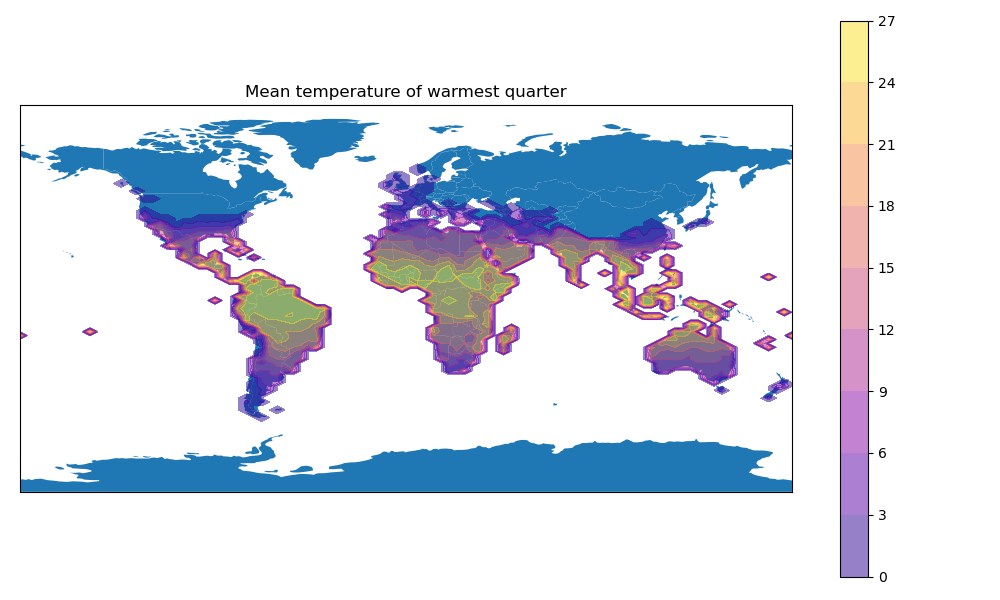
\includegraphics[width=\linewidth]{Images/mean_temp_warm.png}

\end{subfigure}
\begin{subfigure}{.3\linewidth}
  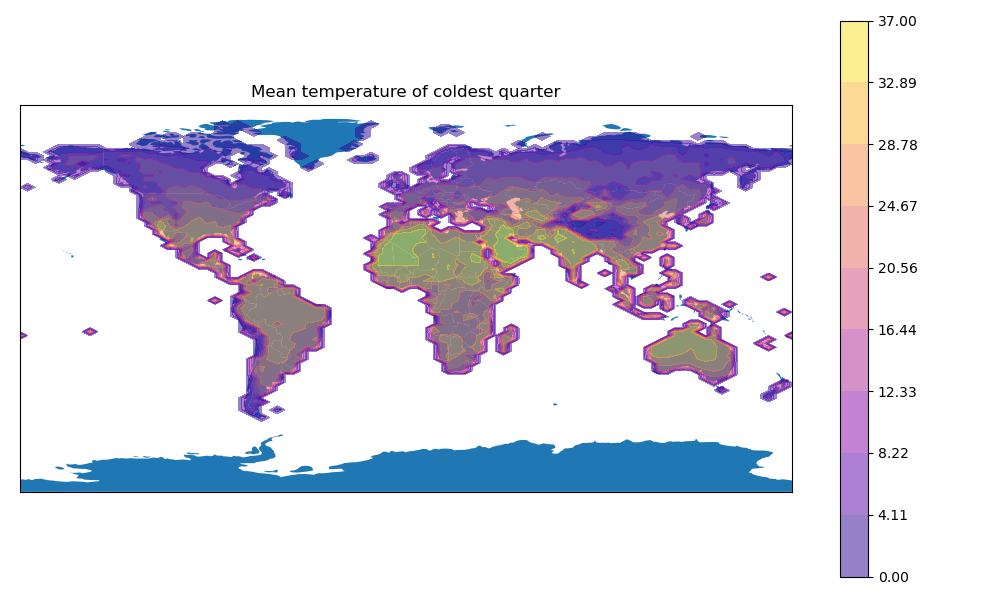
\includegraphics[width=\linewidth]{Images/mean_temp_cold.png} 

\end{subfigure} 

\begin{subfigure}{.3\linewidth}
  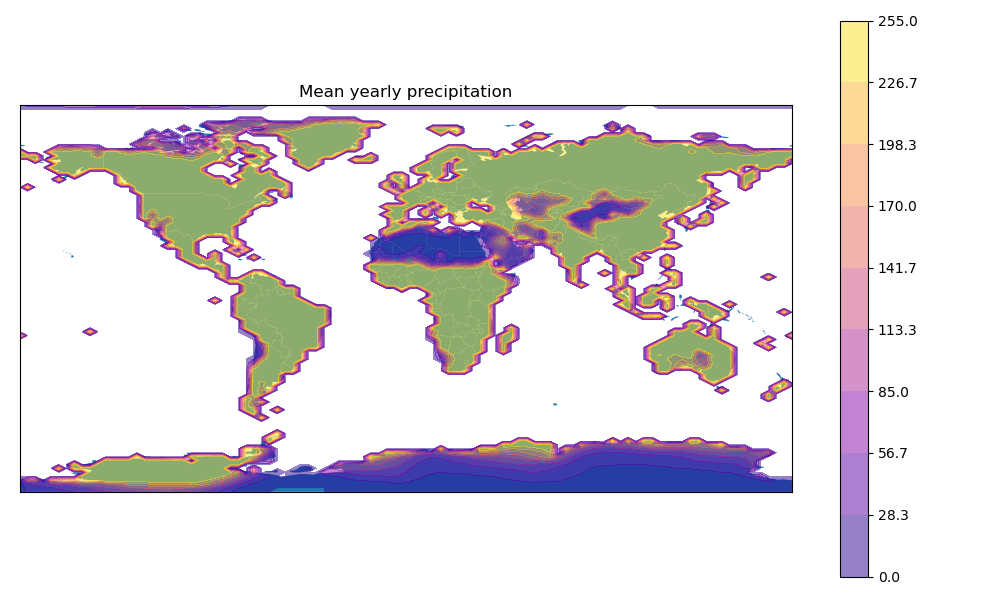
\includegraphics[width=\linewidth]{Images/mean_precip.png}

\end{subfigure}
\begin{subfigure}{.3\linewidth}
  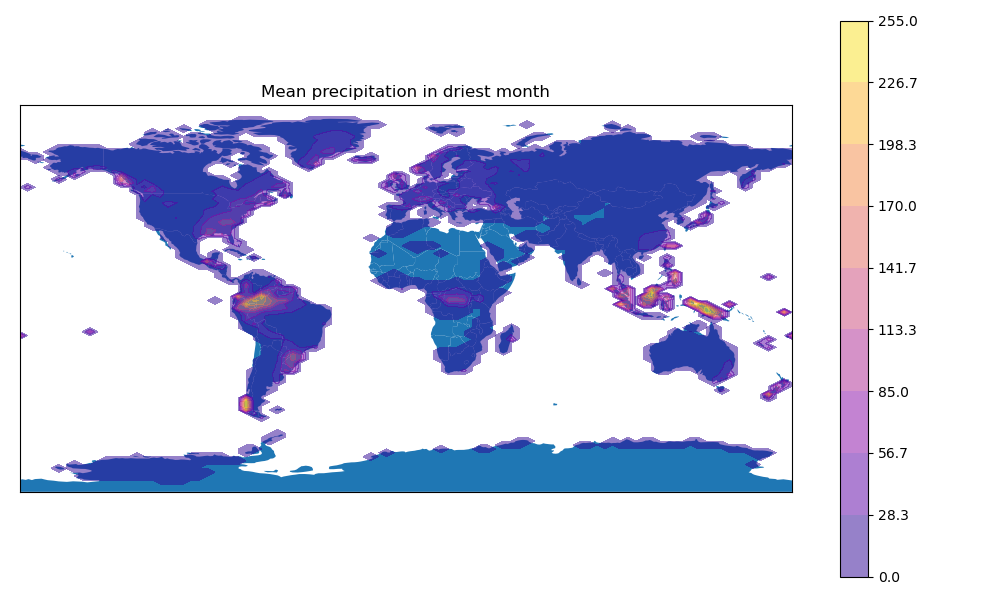
\includegraphics[width=\linewidth]{Images/mean_precip_dry.png}

\end{subfigure}
\begin{subfigure}{.3\linewidth}
  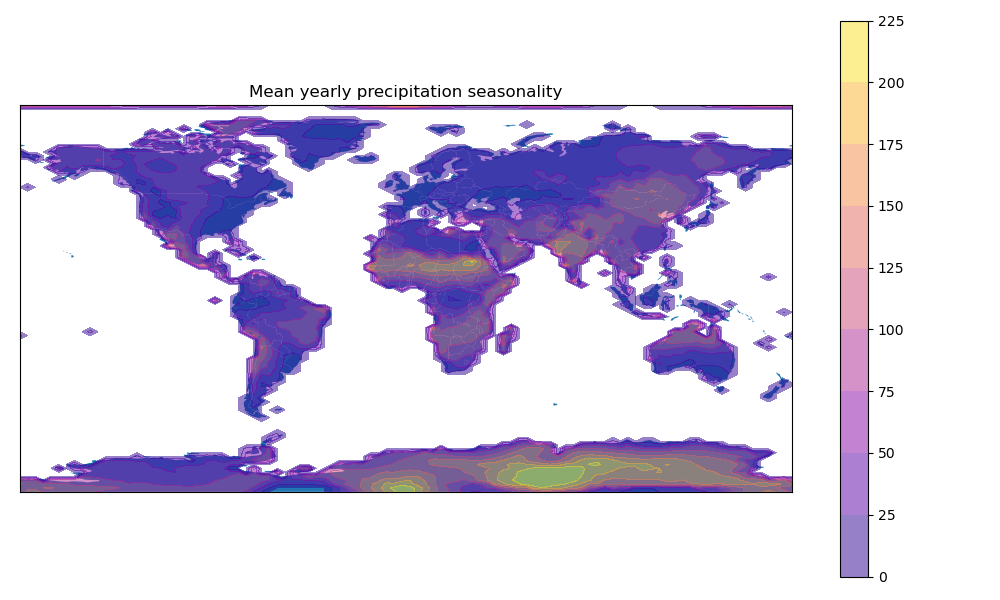
\includegraphics[width=\linewidth]{Images/mean_precip_seasonality.png} 

\end{subfigure} 

\caption{Bio-climatic variables introduced to further train models. (Top) from right to left is the mean yearly temperature range, mean temperature of the warmest quarter, and mean temperature of the coldest quarter.
(Bottom) from right to left is the mean yearly precipitation, mean precipitation in the driest month, and mean precipitation seasonality.}
\label{fig:extra}
\end{figure}

\section{Over estimation of small-distribution species with 8-feature model}\label{appendix:smalldistn}

\begin{figure}[H]
\centering

\begin{subfigure}{.4\linewidth}
  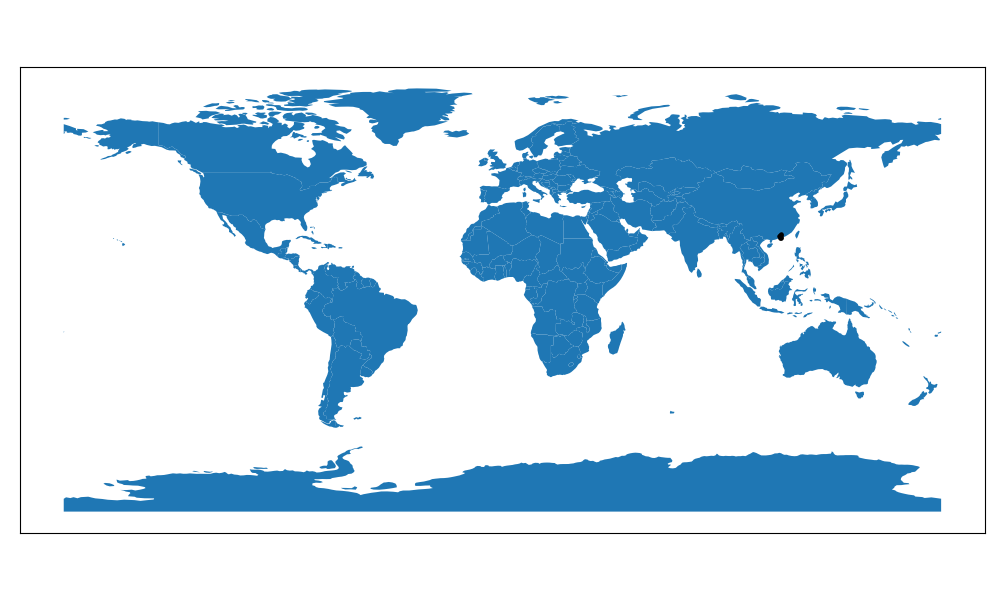
\includegraphics[width=\linewidth]{Images/small_distn_true.png}

\end{subfigure}
\begin{subfigure}{.4\linewidth}
  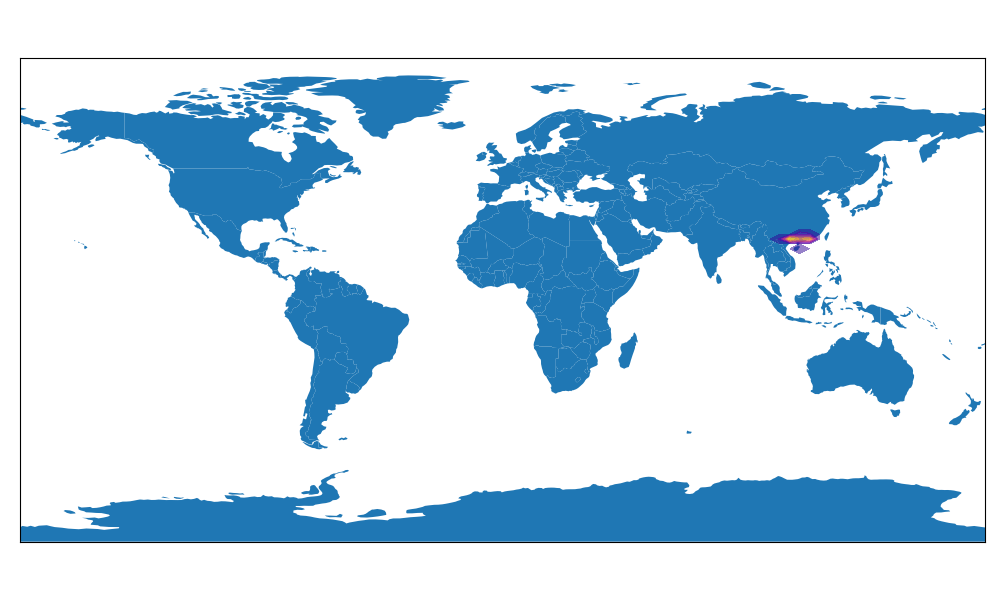
\includegraphics[width=\linewidth]{Images/small_distn_overestimation.png}

\end{subfigure}
\caption{Overestimation of species from the small-population distribution sample (taxon ID 64387) with the use of FFNN trained with bio-climatic variables.}
\end{figure}

\section{Temperature anomaly} \label{appendix:temp-anomaly}

\begin{figure} [H]
    \centering
    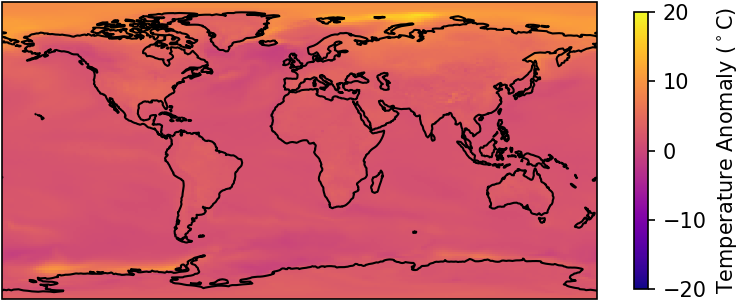
\includegraphics[width=0.5\linewidth]{Images/temp_anomaly.png}
    \caption{Projected yearly average temperature anomaly for 2050 compared to 1984-2014 baseline}
\end{figure}



\section{Arctic Ground Squirrel predicted distribution 8-feature FFNN} \label{appendix:arcticsq}

\begin{figure} [H]
    \centering
\vspace*{-1ex}  
\begin{center}
\textbf{Arctic G. Squirrel predicted distribution + vulnerability}
\end{center}
\vspace*{0ex}
    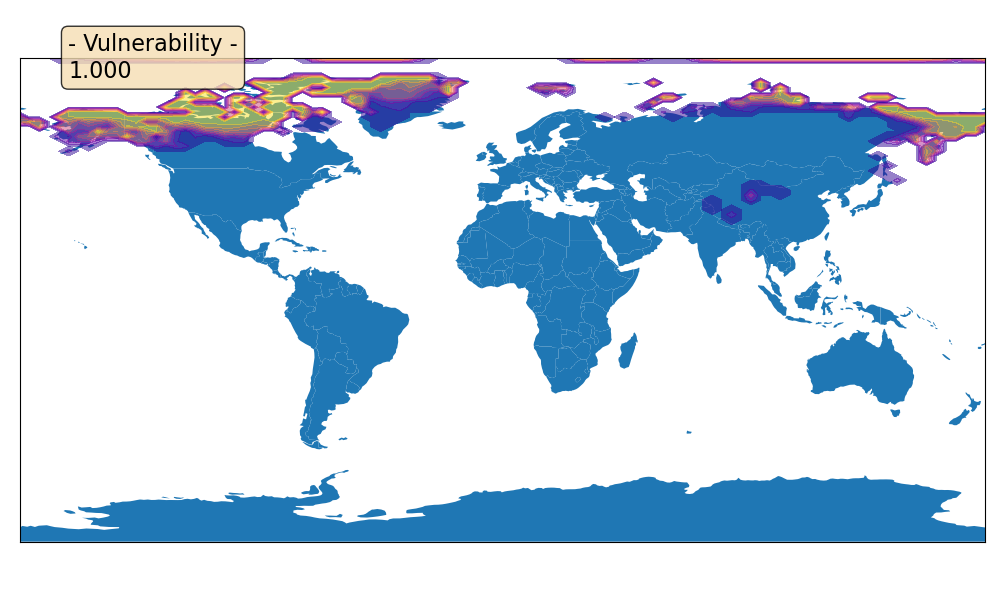
\includegraphics[width=0.5\linewidth]{Images/arctic squirrel vulnerability.png}
    \caption{8-feature FFNN population distribution prediction for the most vulnerable species in the data-set (\emph{Arctic Ground Squirrel}) alongside its scaled vulnerability score, 1.0, indicating the highest net-affect as a result of temperature anomaly.}
    \label{fig:arcticsq}
\end{figure}
